\section{ХОД РАБОТЫ}

\subsection{Текст задания}

Разработанная программа должна выводить на экран в виде гистограммы зависимость
числа регистрируемых событий в выбранном журнале от времени суток (с точностью до часа),
в котором была выполнена регистрация.

\subsection{Детали реализации программы}

Процесс работы программы можно разделить на следующие этапы:

\begin{enumerate}
\item получение данных о числе событий из системного журнала;
\item нормировка полученных данных;
\item вывод данных в виде гистограммы на экран.
\end{enumerate}

Для хранения данных о событиях будем использовать массив чисел с плавающей точкой,
состоящий из 24 элементов (соостветствут числу часов в сутках),
инициализированных нулем.
С помощью командлетов \textit{Get-EventLog} и \textit{Foreach-Object} заполним
массив данными о числе 
регистрируемых событий, приходящихся на каждый час суток, как показано 
на рисунке~\ref{lst:get_data}.

\begin{lstlisting}[caption=Получение данных о числе событий,label=lst:get_data]
 $freq = ,0 * 24
 
 Get-Eventlog -Logname $eventLog | Foreach-Object {
   $h = $_.TimeGenerated.Hour
   $freq[$h]++
 }
\end{lstlisting}

После этого производится нормировка данных массива --- вычисление относительной 
частоты регистрации событий в час.
Выполнение нормировки необходимо для корректного построения гистограммы 
(в соответствии с теорией вероятности).
Для выполнения нормировки достаточно каждый элемент массива (число событий,
приходящихся на данный час) разделить на сумму значений элементов 
массива (общее число событий), как показано на рисунке~\ref{lst:enumerate_data}.

\begin{lstlisting}[caption=Нормировка данных о числе событий,label=lst:enumerate_data]
 $total = 0
 ForEach ($val in $freq) { $total += $val }
 For ($i = 0; $i -lt $freq.Length; $i++) { $freq[$i] /= $total }
\end{lstlisting}

После нормировки можно делать построение и вывод гистограммы на экран.
Эту задачу выполняет функция \textit{Write-Histogram}, 
приведенная на рисунке~\ref{lst:write_data}.

\begin{lstlisting}[caption=Функция построения гистограммы \textit{Write-Histogram},label=lst:write_data]
 Function Write-Histogram ([double[]] $freq, [int] $bar_width) {
     $max_freq = ($freq | Measure-Object -Max).Maximum
     if ($max_freq -eq 0) { $max_freq = 1 } 
 
     For ($i = 0; $i -lt $freq.Length; $i++) {
       $cur_start_time = "{0,2}:{1,0}" -f $i, "00"
       $cur_freq = $freq[$i]
       $cur_num_filled = $bar_width * ($cur_freq / $max_freq)
       
       $cur_bar = "["
       
       $cur_bar += "#" * $cur_num_filled
       $cur_bar += "-" * ($bar_width - $cur_num_filled)
       $cur_bar += "]"
       
       $cur_percent = "{0:N2}%" -f ($cur_freq * 100)
       Write-Host "$cur_start_time $cur_bar $cur_percent"
     }
 }
\end{lstlisting}

Данная функция принимает в качестве аргументов массив относительных 
частот событий и число, определяющее максимальную длину каждого столбца
гистограммы. Результатом работы данной функции является набор строк вида 
<<\textit{час} [\#...\#-...-] (\textit{процент})>>,
где под \textit{часом} понимается время суток,
в течение которого было зарегистрировано событие,
а под \textit{процентом} --- относительная
частота зарегистрированных событий за данный час. 

Результат работы программы приведен на рисунке~\ref{fig:screen}.

\begin{figure}[h!]
  \centering
  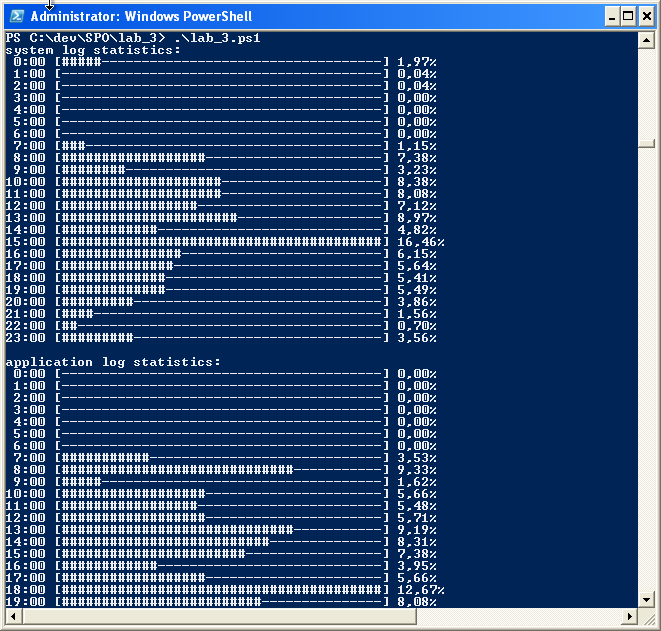
\includegraphics[width=150mm]{img/screen}
  \caption{Результат работы программы}\label{fig:screen}
\end{figure}

Исходный код разработанной программы расположен в приложении А.

\newpage
